% Options for packages loaded elsewhere
\PassOptionsToPackage{unicode}{hyperref}
\PassOptionsToPackage{hyphens}{url}
%
\documentclass[
  12pt,
]{article}
\usepackage{amsmath,amssymb}
\usepackage{iftex}
\ifPDFTeX
  \usepackage[T1]{fontenc}
  \usepackage[utf8]{inputenc}
  \usepackage{textcomp} % provide euro and other symbols
\else % if luatex or xetex
  \usepackage{unicode-math} % this also loads fontspec
  \defaultfontfeatures{Scale=MatchLowercase}
  \defaultfontfeatures[\rmfamily]{Ligatures=TeX,Scale=1}
\fi
\usepackage{lmodern}
\ifPDFTeX\else
  % xetex/luatex font selection
\fi
% Use upquote if available, for straight quotes in verbatim environments
\IfFileExists{upquote.sty}{\usepackage{upquote}}{}
\IfFileExists{microtype.sty}{% use microtype if available
  \usepackage[]{microtype}
  \UseMicrotypeSet[protrusion]{basicmath} % disable protrusion for tt fonts
}{}
\makeatletter
\@ifundefined{KOMAClassName}{% if non-KOMA class
  \IfFileExists{parskip.sty}{%
    \usepackage{parskip}
  }{% else
    \setlength{\parindent}{0pt}
    \setlength{\parskip}{6pt plus 2pt minus 1pt}}
}{% if KOMA class
  \KOMAoptions{parskip=half}}
\makeatother
\usepackage{xcolor}
\usepackage[margin=1in]{geometry}
\usepackage{graphicx}
\makeatletter
\def\maxwidth{\ifdim\Gin@nat@width>\linewidth\linewidth\else\Gin@nat@width\fi}
\def\maxheight{\ifdim\Gin@nat@height>\textheight\textheight\else\Gin@nat@height\fi}
\makeatother
% Scale images if necessary, so that they will not overflow the page
% margins by default, and it is still possible to overwrite the defaults
% using explicit options in \includegraphics[width, height, ...]{}
\setkeys{Gin}{width=\maxwidth,height=\maxheight,keepaspectratio}
% Set default figure placement to htbp
\makeatletter
\def\fps@figure{htbp}
\makeatother
\setlength{\emergencystretch}{3em} % prevent overfull lines
\providecommand{\tightlist}{%
  \setlength{\itemsep}{0pt}\setlength{\parskip}{0pt}}
\setcounter{secnumdepth}{-\maxdimen} % remove section numbering
\ifLuaTeX
  \usepackage{selnolig}  % disable illegal ligatures
\fi
\IfFileExists{bookmark.sty}{\usepackage{bookmark}}{\usepackage{hyperref}}
\IfFileExists{xurl.sty}{\usepackage{xurl}}{} % add URL line breaks if available
\urlstyle{same}
\hypersetup{
  pdftitle={Final Report},
  pdfauthor={Daniel Malone and Margo La Clair},
  hidelinks,
  pdfcreator={LaTeX via pandoc}}

\title{Final Report}
\author{Daniel Malone and Margo La Clair}
\date{2023-12-03}

\begin{document}
\maketitle

\hypertarget{i.-topic}{%
\subsubsection{I. Topic}\label{i.-topic}}

\setlength\parindent{24pt}

~~~~~Crime is a complex topic, and there is no academic (or popular)
consensus on either the reasons for criminal behavior or the appropriate
interventions to curtail such behavior. One theoretical intervention is
reducing crime via changing the ``built environment''---incorporating a
spatial element to crime. This broadly ranges from land policy (zoning)
to more targeted planning and landscaping interventions that focus on
surveillance, access control, and target hardening (see Carter et al,
2003 and Katyal, 2002). The latter has a long history: in 1285, King
Edward I decreed that bushes should be removed along highways to deter
robbery (Anderson et al., 2013). Controlling crime via the built
environment is an attractive policy, as a zoning change might be more
efficient (or more politically palatable) than throwing more resources
into enforcement and punishment.

Theoretically, exclusionary zoning practices can help create
concentrations of poverty, which could create an environment where crime
is more likely. The actual academic literature on the interaction
between land policy and crime do find some associations (generally
surrounding the debate over the merits of mixed-use residential zoning),
but there are few empirical studies (Anderson et al.~blame this on a
lack of data). One of the more influential non-empirical works is Jane
Jacobs' 1961 book \emph{The Death and Life of Great American Cities},
which advocated for including commercial businesses in residential areas
to reduce crime. Empirical investigations produced mixed results.
Anderson et al.'s (2013) study of Los Angeles finds that commercial-only
zoned areas are associated with higher crime rates, and that zoning
changes that including residential parcels in prior commercial-zoned
areas is associated with a reduction in crime. Browning et al.~(2010)
finds a curvilinear association between density -- both commercial and
residential -- and assault and homicide.

The current housing crisis has caused many cities, and even states, to
either consider or enact zoning reform. These reforms (such as the 2023
state-wide reforms in Montana) often effectively eliminate single-family
residential zoning by allowing multi-family development (ranging from
`granny suites' to triplexes) in what was formally single-family
residential neighborhoods. This push is also coming from the White
House; the Biden infrastructure bill includes incentives for municipal
zoning reform. Are these zoning changes associated with any changes in
crime, at either the state or individual municipal level?

\hypertarget{ii.-data-sources-and-notes-on-data-limitations}{%
\subsubsection{II. Data Sources and Notes on Data
Limitations}\label{ii.-data-sources-and-notes-on-data-limitations}}

\setlength\parindent{24pt}

~~~~~Our primary data comes from two sources: the FBI and the University
of California, Berkely. We use the FBI's crime data to observe crime at
a state and city level for the years 2020-2022. This dataset has
variables on population, total crime, and a further breakdown of types
of crime (generally sorted into personal, social, and property). We then
merge the University of California, Berkeley's data on municipal-level
zoning reform for the year 2021 onto this crime dataset. We also used
secondary data sources to merge on state-wide zoning changes
(Meyershohn). Unemployment data on a state-wide level was provided by
the United States Department of Agriculture.

Due to data limitations from the FBI dataset, we are restricted to the
years 2020 to 2022. Furthermore, the Covid-19 pandemic deeply impacted
the reporting at a state-wide level. For example, California does not
have consistent data from 2020-2022. None of the cities in California
report crime statistics for 2020. If we had additional years of crime
data before the Covid-19 disruptions, we might have more options for
dealing with the missing data (i.e.~able to impute these missing values)
. However, since our dataset is so limited, we had to exclude cities
that had incomplete reporting data. After we filtered for having crime
statistics in all three years, we are left with 44 states. We note that
the distribution of cities within these states is not consistent. Some
states, such as Michigan, are very well documented; while others, like
Illinois and Pennsylvania have one and two reporting cities,
respectively. Future research might look for more data, in order to
better capture the prior trends, as well as look at the long-term impact
of zoning changes.

Further, the crime statistics used are on a agency wide scale; they are
notably not using the more widely used FIPS code system. This makes it
difficult to append additional datasets for use as control data, since
many datasets use FIPS codes, and are typically not on a city to city
basis. Additionally, since housing reform happened so recently, data for
certain varibles which would have been useful as control variables, such
as poverty rates and educational attainment, are simply not available.
The econometric analysis will therefore utilize state and year fixed
effects to control for geographic variation.

\hypertarget{iii.-data-cleaning}{%
\subsubsection{III. Data Cleaning}\label{iii.-data-cleaning}}

\setlength\parindent{24pt}

~~~~~The data cleaning processes consisted of merging the three years of
FBI data and converting it into tidy format. Of particular note is the
FBI statistics for the year 2022, which was formatted slightly
differently from the 2021 and 2020 data sets. All the information was in
the right place, so to speak, but there were unseen differences between
the column names of the datasets, and some of the labels were a row
above their location in the other datasets, which created a small
challenge when merging. This was resolved by manually entering the
offending names to the correct location and then setting the column
names of the 2022 dataset equal to the column names of the larger
2021-2020 dataset, and then merging.

We determined which cities had data for all three years of our event
study and filtering for only those cities. We then merged on the zoning
data, which we had cleaned. Due to the comparatively low number of
cities who passed zoning reform in 2021, we were able to visually
inspect the University of California, Berkeley's summaries to ensure
that these laws involved the loosening of zoning - not increasing zoning
restrictions. This merged file comprises our master dataset. Then, we
merged on data on state-wide zoning changes to our master dataset. Only
Oregon and Maine passed state-wide zoning reforms during our limited
time span: Oregon in 2021 and Maine in 2022. We recognize that, due to
data limitations, we cannot form any conclusions about the impact of
this reform in these states.

\hypertarget{iv.-data-transformations}{%
\subsubsection{IV. Data
Transformations}\label{iv.-data-transformations}}

\setlength\parindent{24pt}

~~~~~We created a log transformed variable for the population per city.
This was done to avoid heavy skew in the case, as the range of
populations per city in the United States can vary from the hundreds to
the millions and, naturally, have varying numbers of criminal citations.
To avoid problems in interpreting the data visually, we created an
additional variable which log-transformed population. It is easier to
interpret crime per capita rather than total numbers of citations in a
city, so we created additional variables which calculated the total,
property, personal and societal crime per capita, as well as multiplying
these values by 1,000 to report the crime rate per 1,000 people. Some of
the municipalities in our dataset have very low populations, so there
are some extreme outliers for these calculations.

We also created variables which record the average total crime rate for
each agency and state. For the state-level variables, we averaged the
crime rate (broken up into total crime, crimes against society, crimes
against persons, and crimes against property) across the cities in that
state. This was done so they may be used during econometric analysis as
dependent variables, as well as for the graphics. The cities enacting
zoning reforms may be experiencing more crime than areas which are not
receiving reforms, and including the average crime rate for each agency
would control for differences in preexisting crime rates. Additionally,
variables which recorded the average crime rate for each sub-categories
defined by the FBI (crime against persons, society and property) were
similarly generated.

We created additional dummy variables which reported whether the city in
question enacted a zoning reform and whether a state in question had
zoning reform in that year as well.

\hypertarget{v.-plots-and-remarks}{%
\subsubsection{V. Plots and Remarks}\label{v.-plots-and-remarks}}

The following map shows the percent change in mean total crime rate for
the cities in all states (that we have data on) for 2020-2022. For ease
of visibility, this is aggregated up to the state level. Note that
Pennsylvania is a clear outlier. Given the above-noted issues with our
data due to Covid-19 reporting issues, our following maps remove
Pennsylvania for ease of visually differentiating crime rate variation.
Maps that include Pennsylvania are included in the Plots sub-folder on
Github.

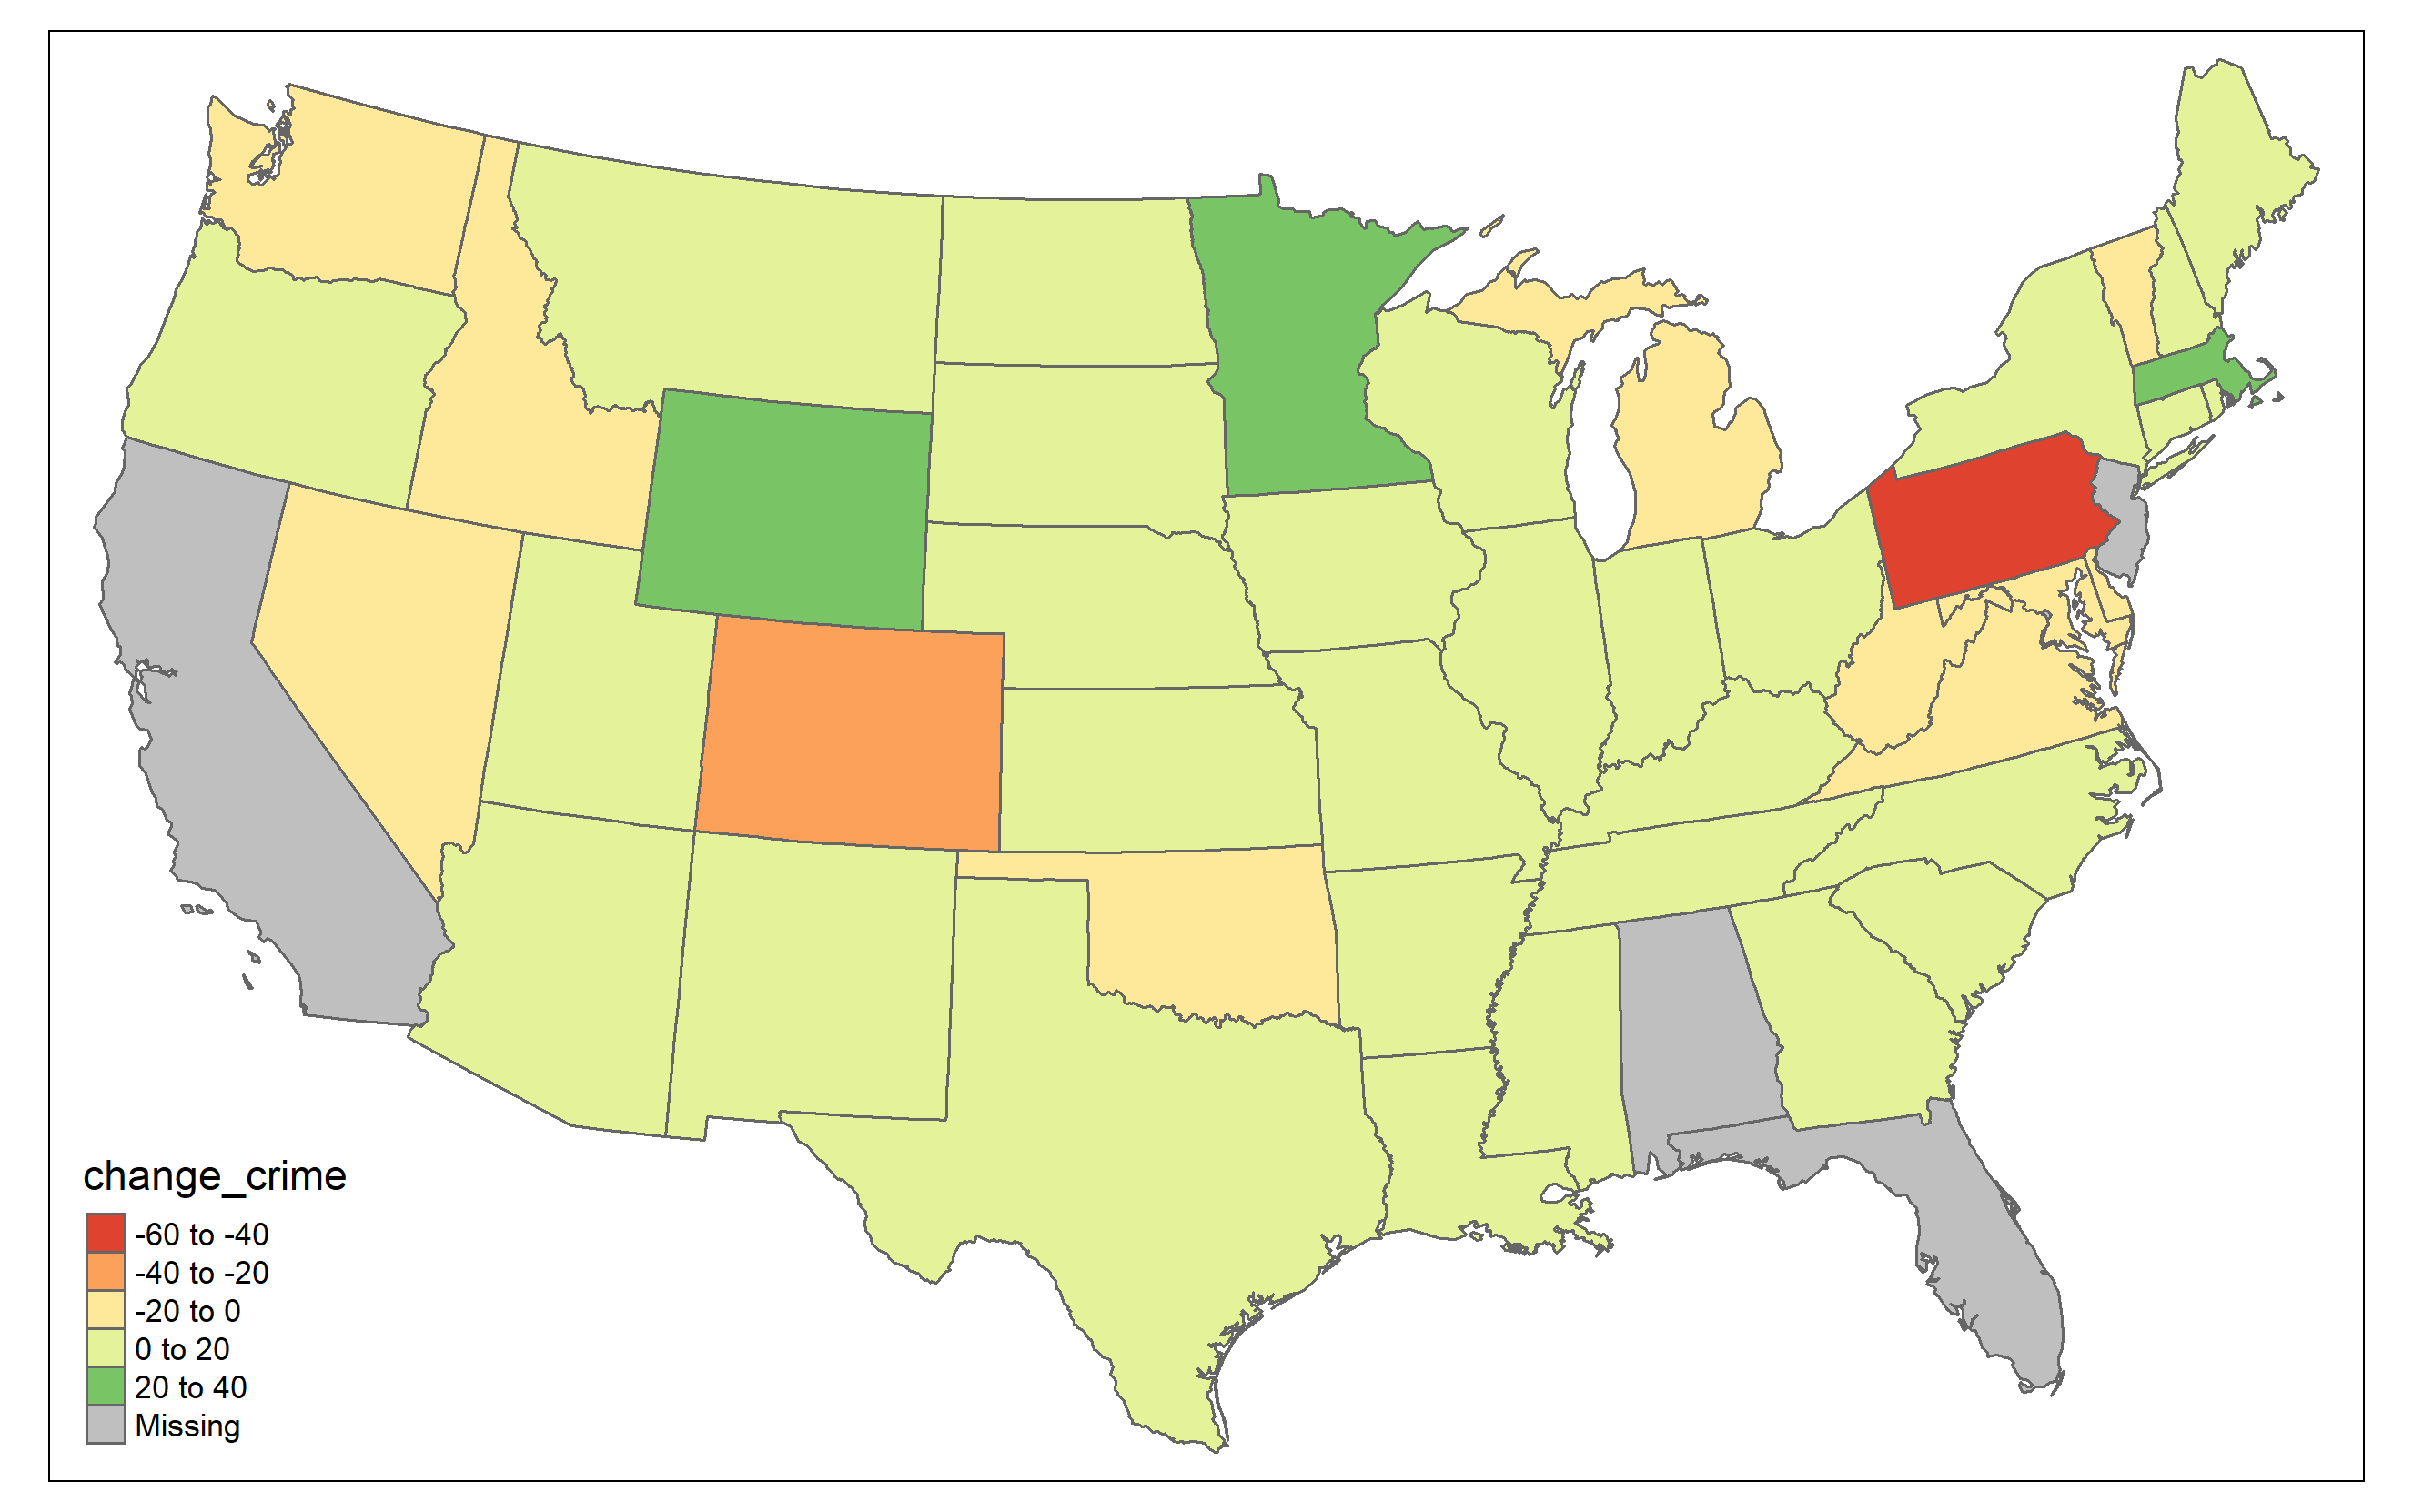
\includegraphics{Plots/States.png}

The map below shows the percent change in mean crime rate but removes
Pennsylvania.

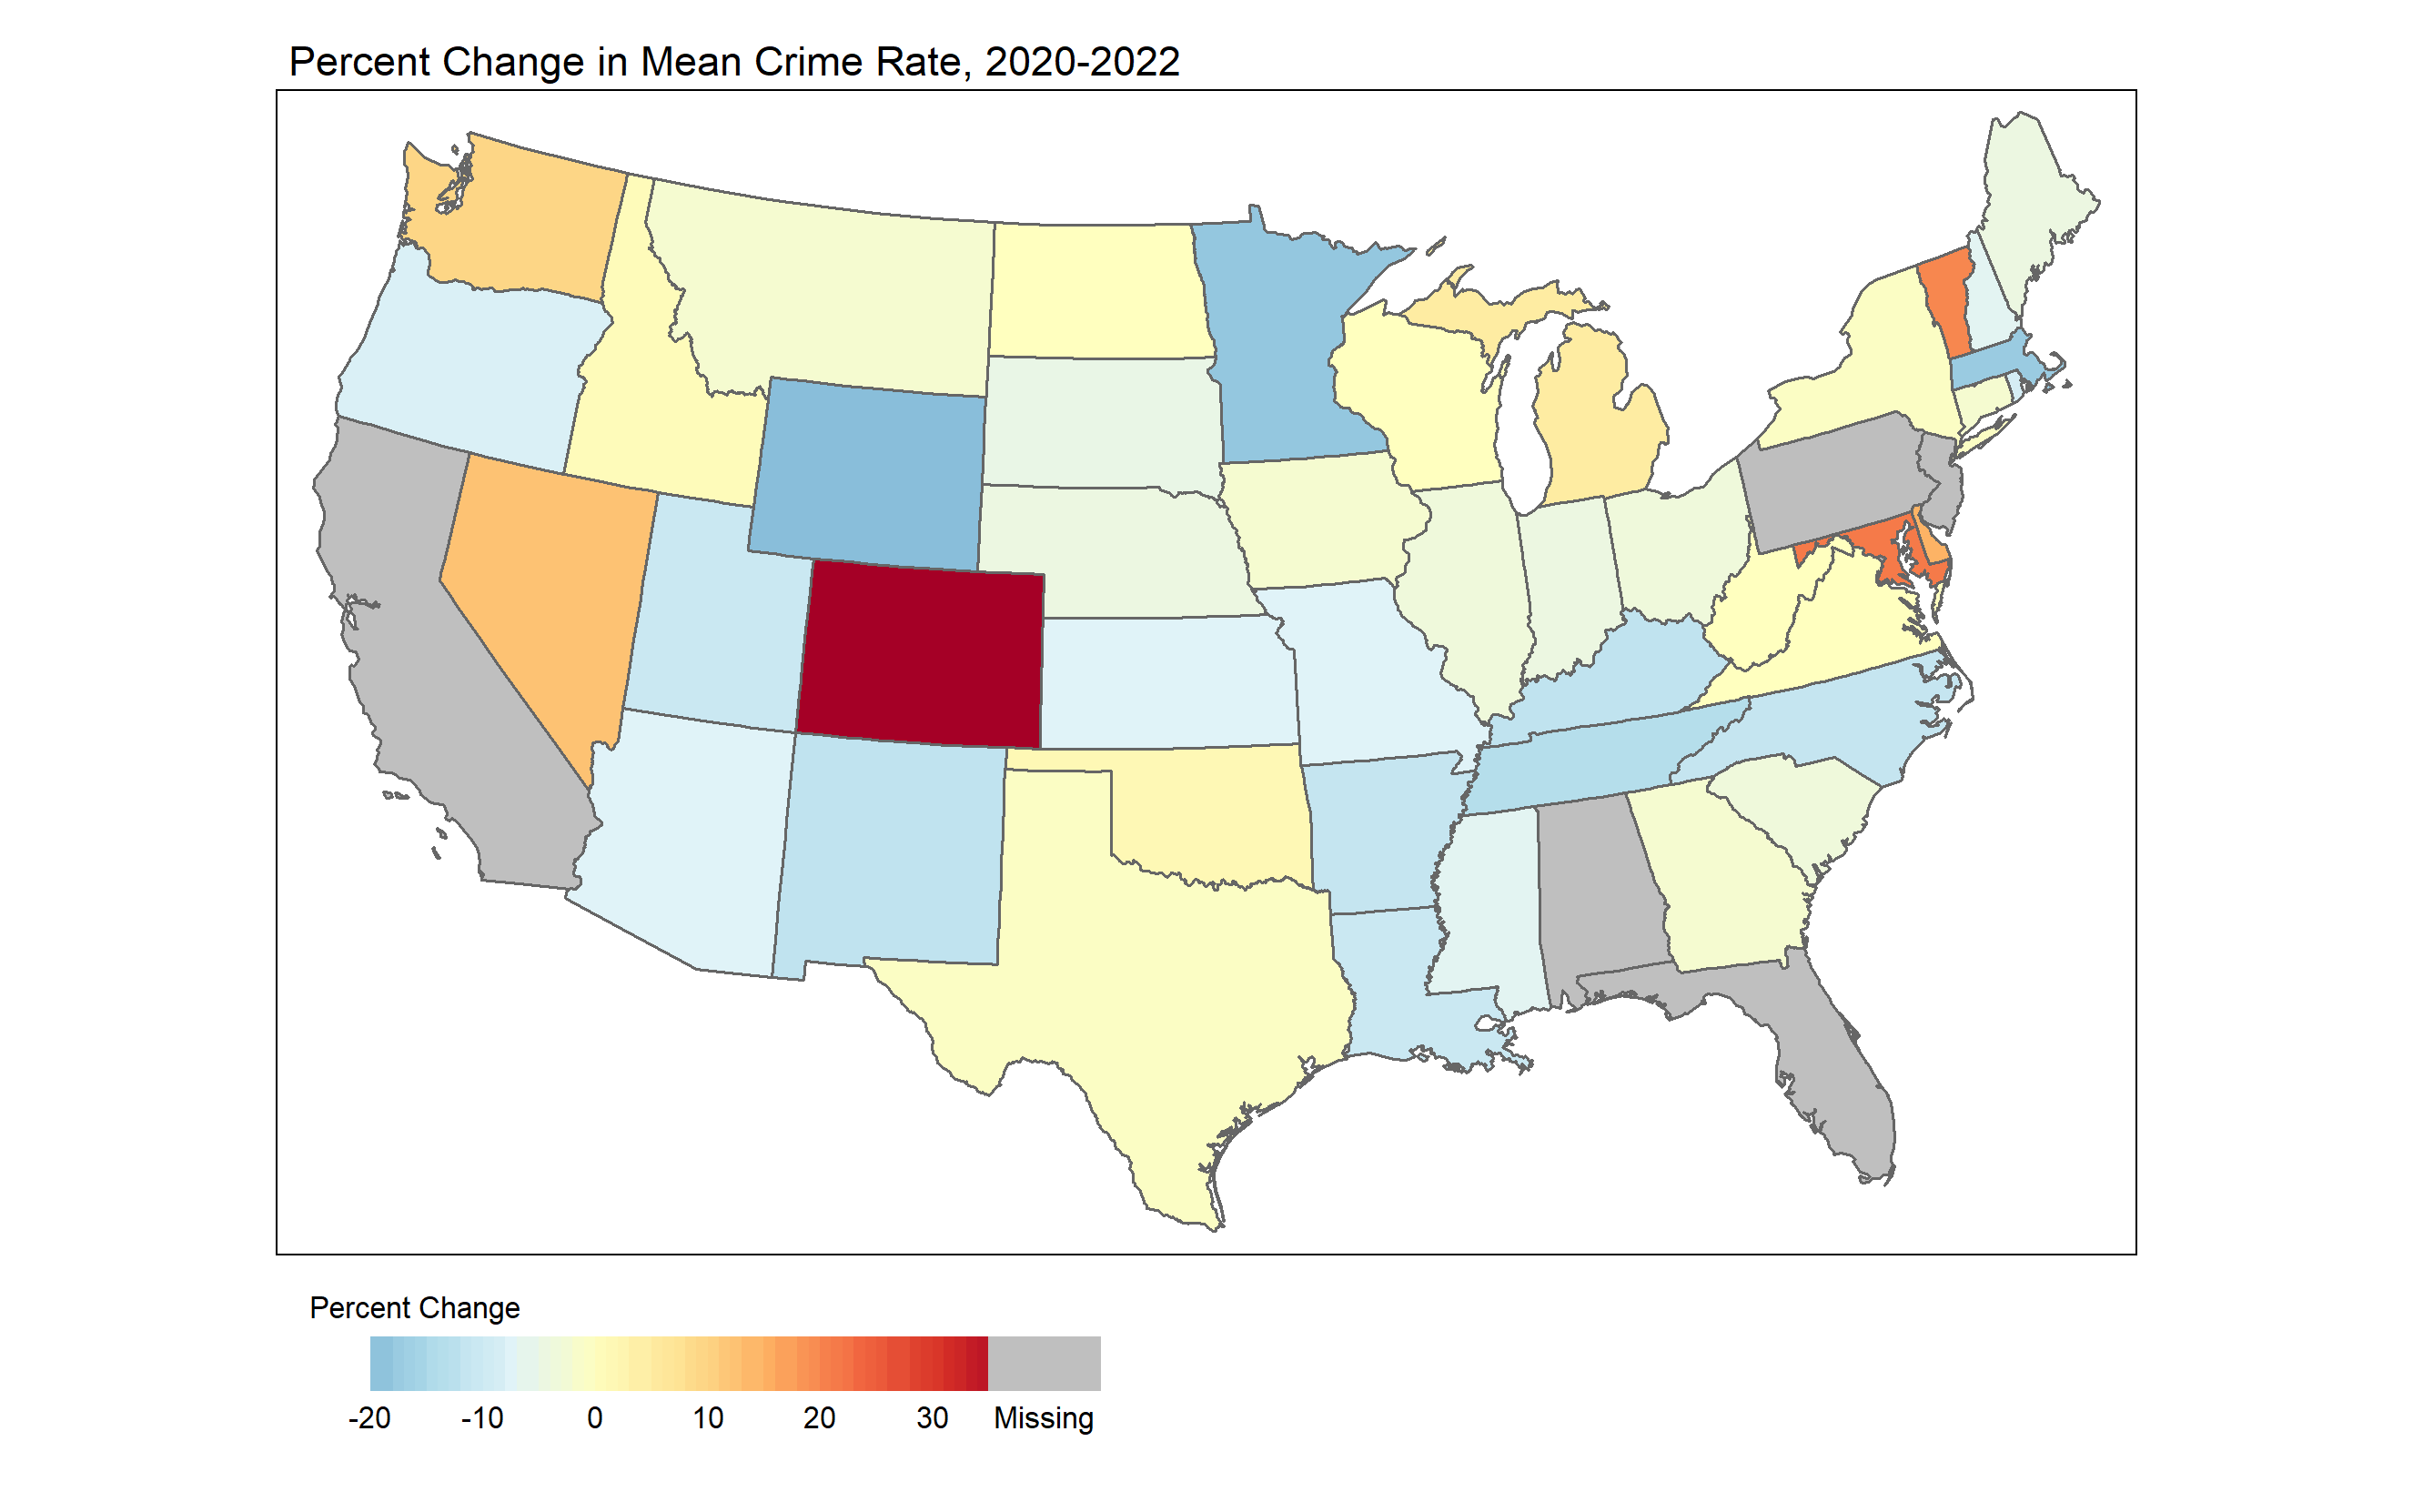
\includegraphics{Plots/States_noPA.png}

The following series of maps show the percent change in mean crime rates
for crimes against persons and property. Note that all remove
Pennsylvania for ease of visual variation.

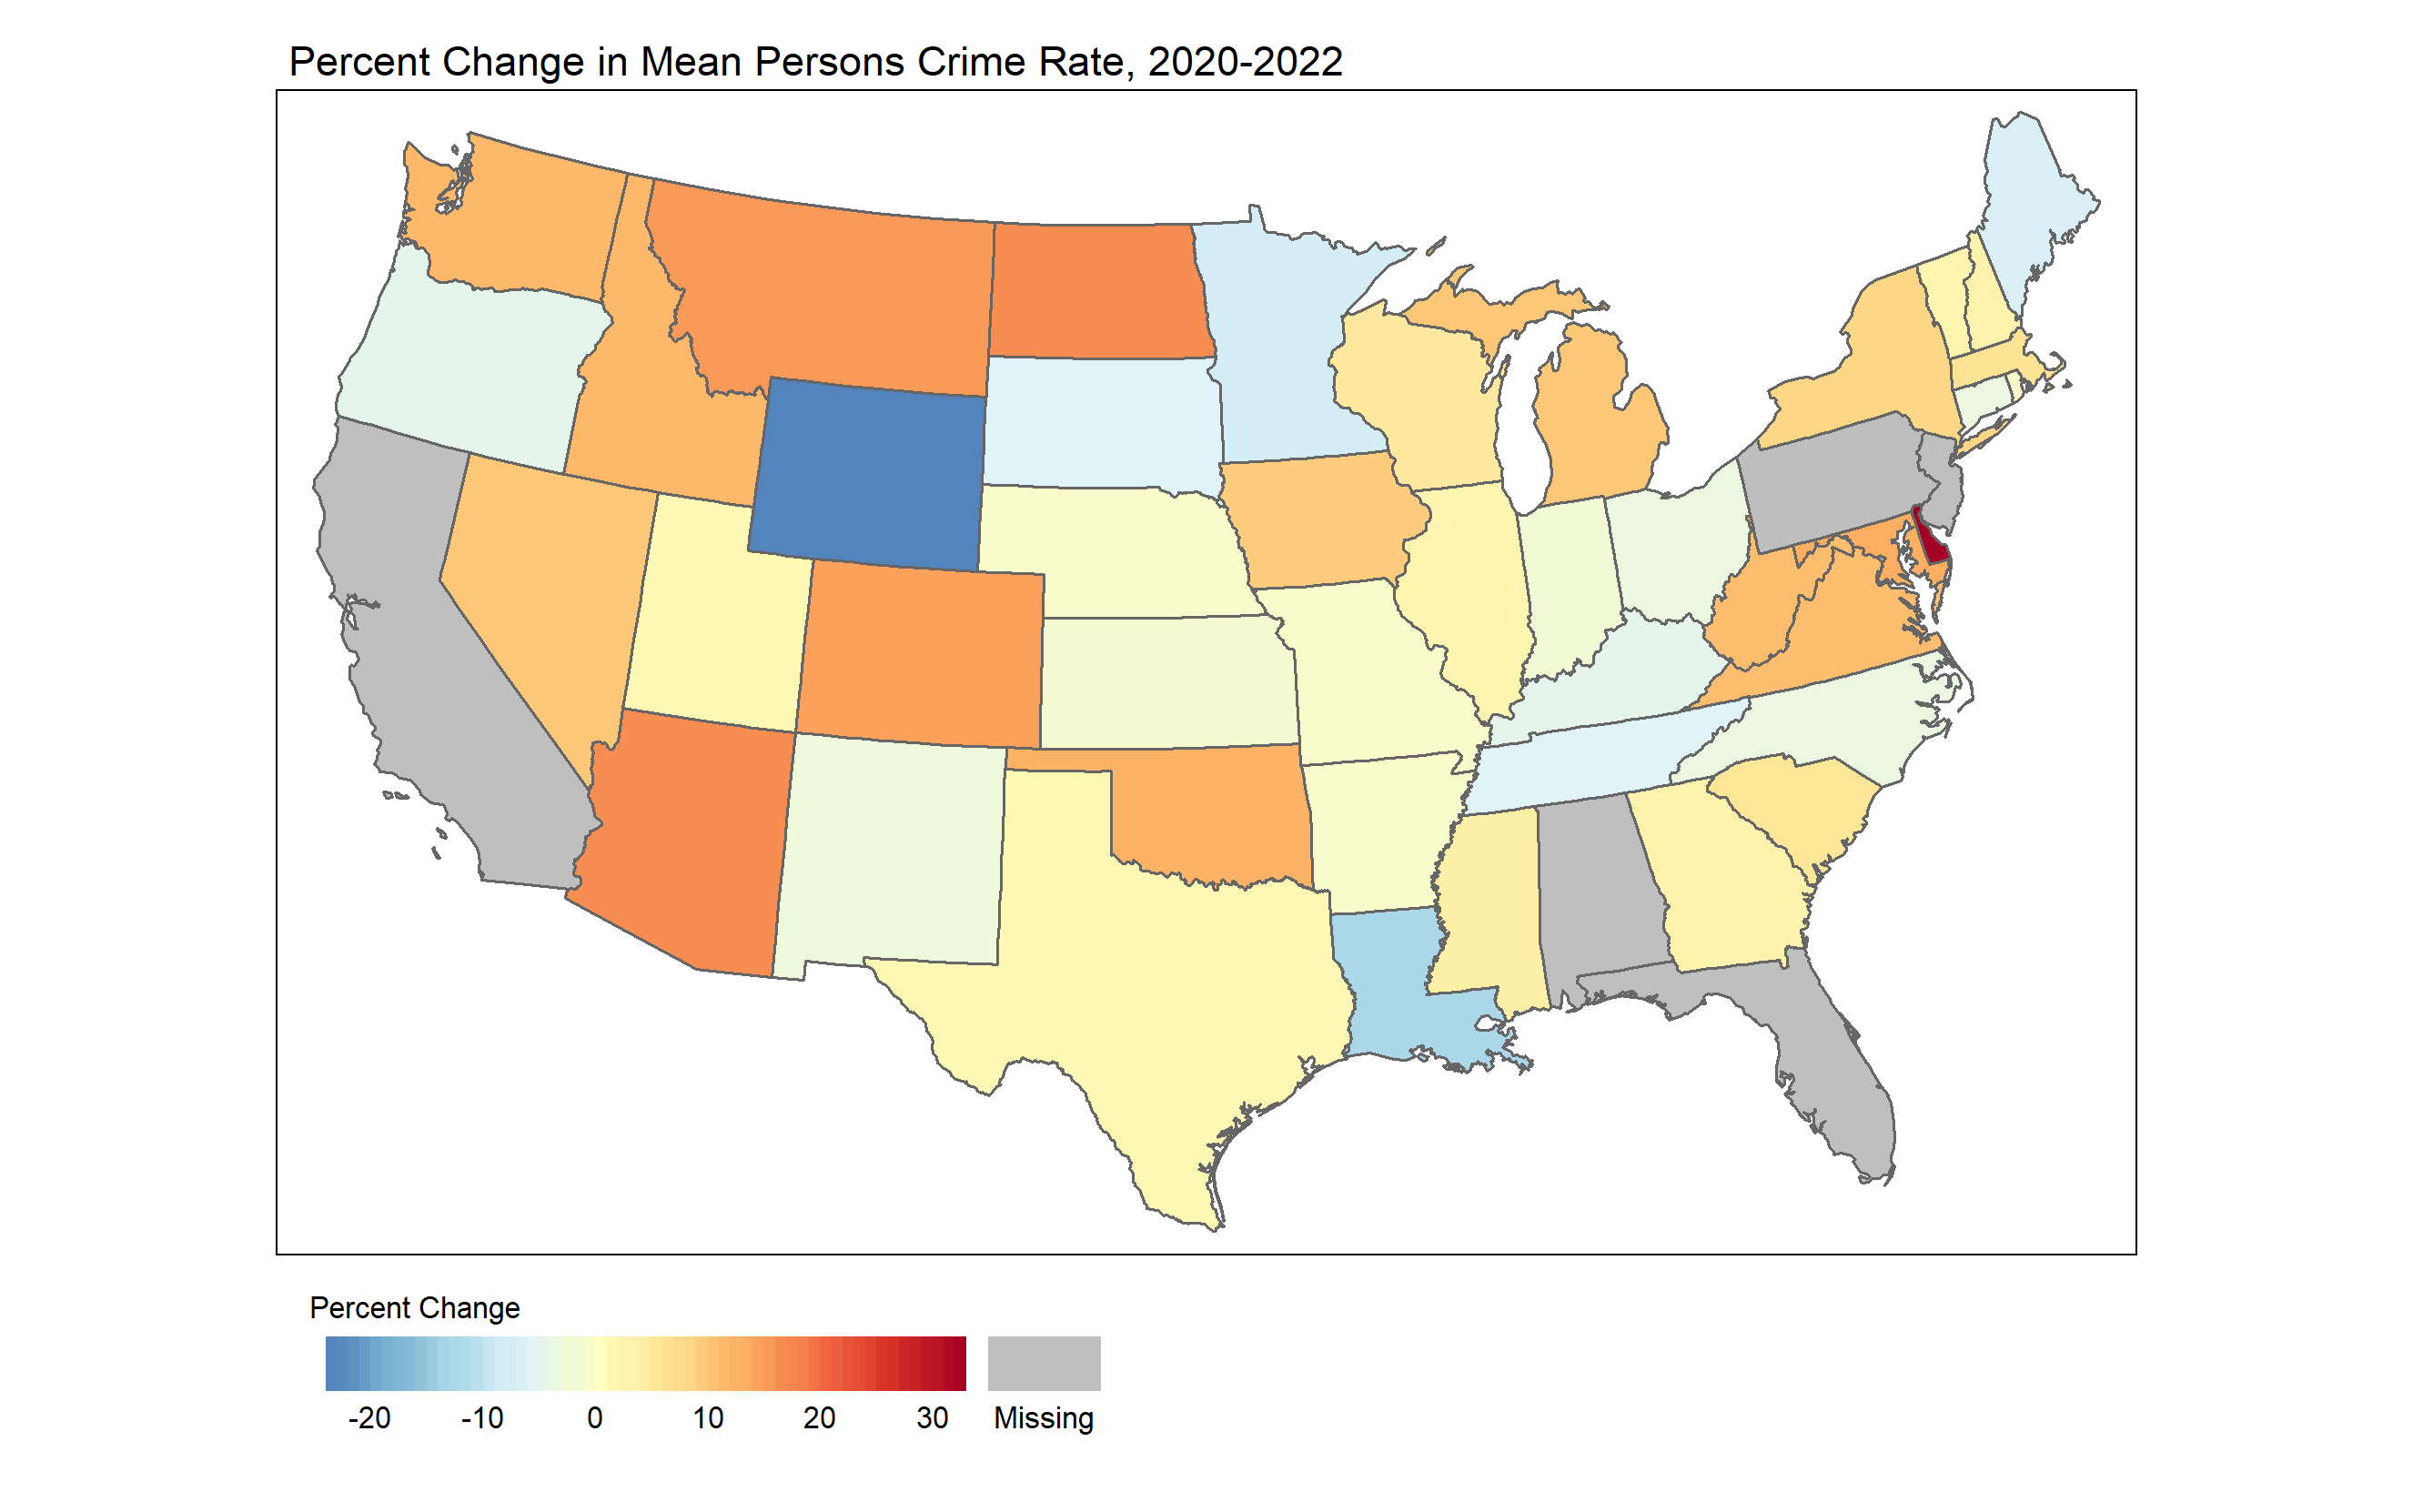
\includegraphics{Plots/States_Person_noPA.png}

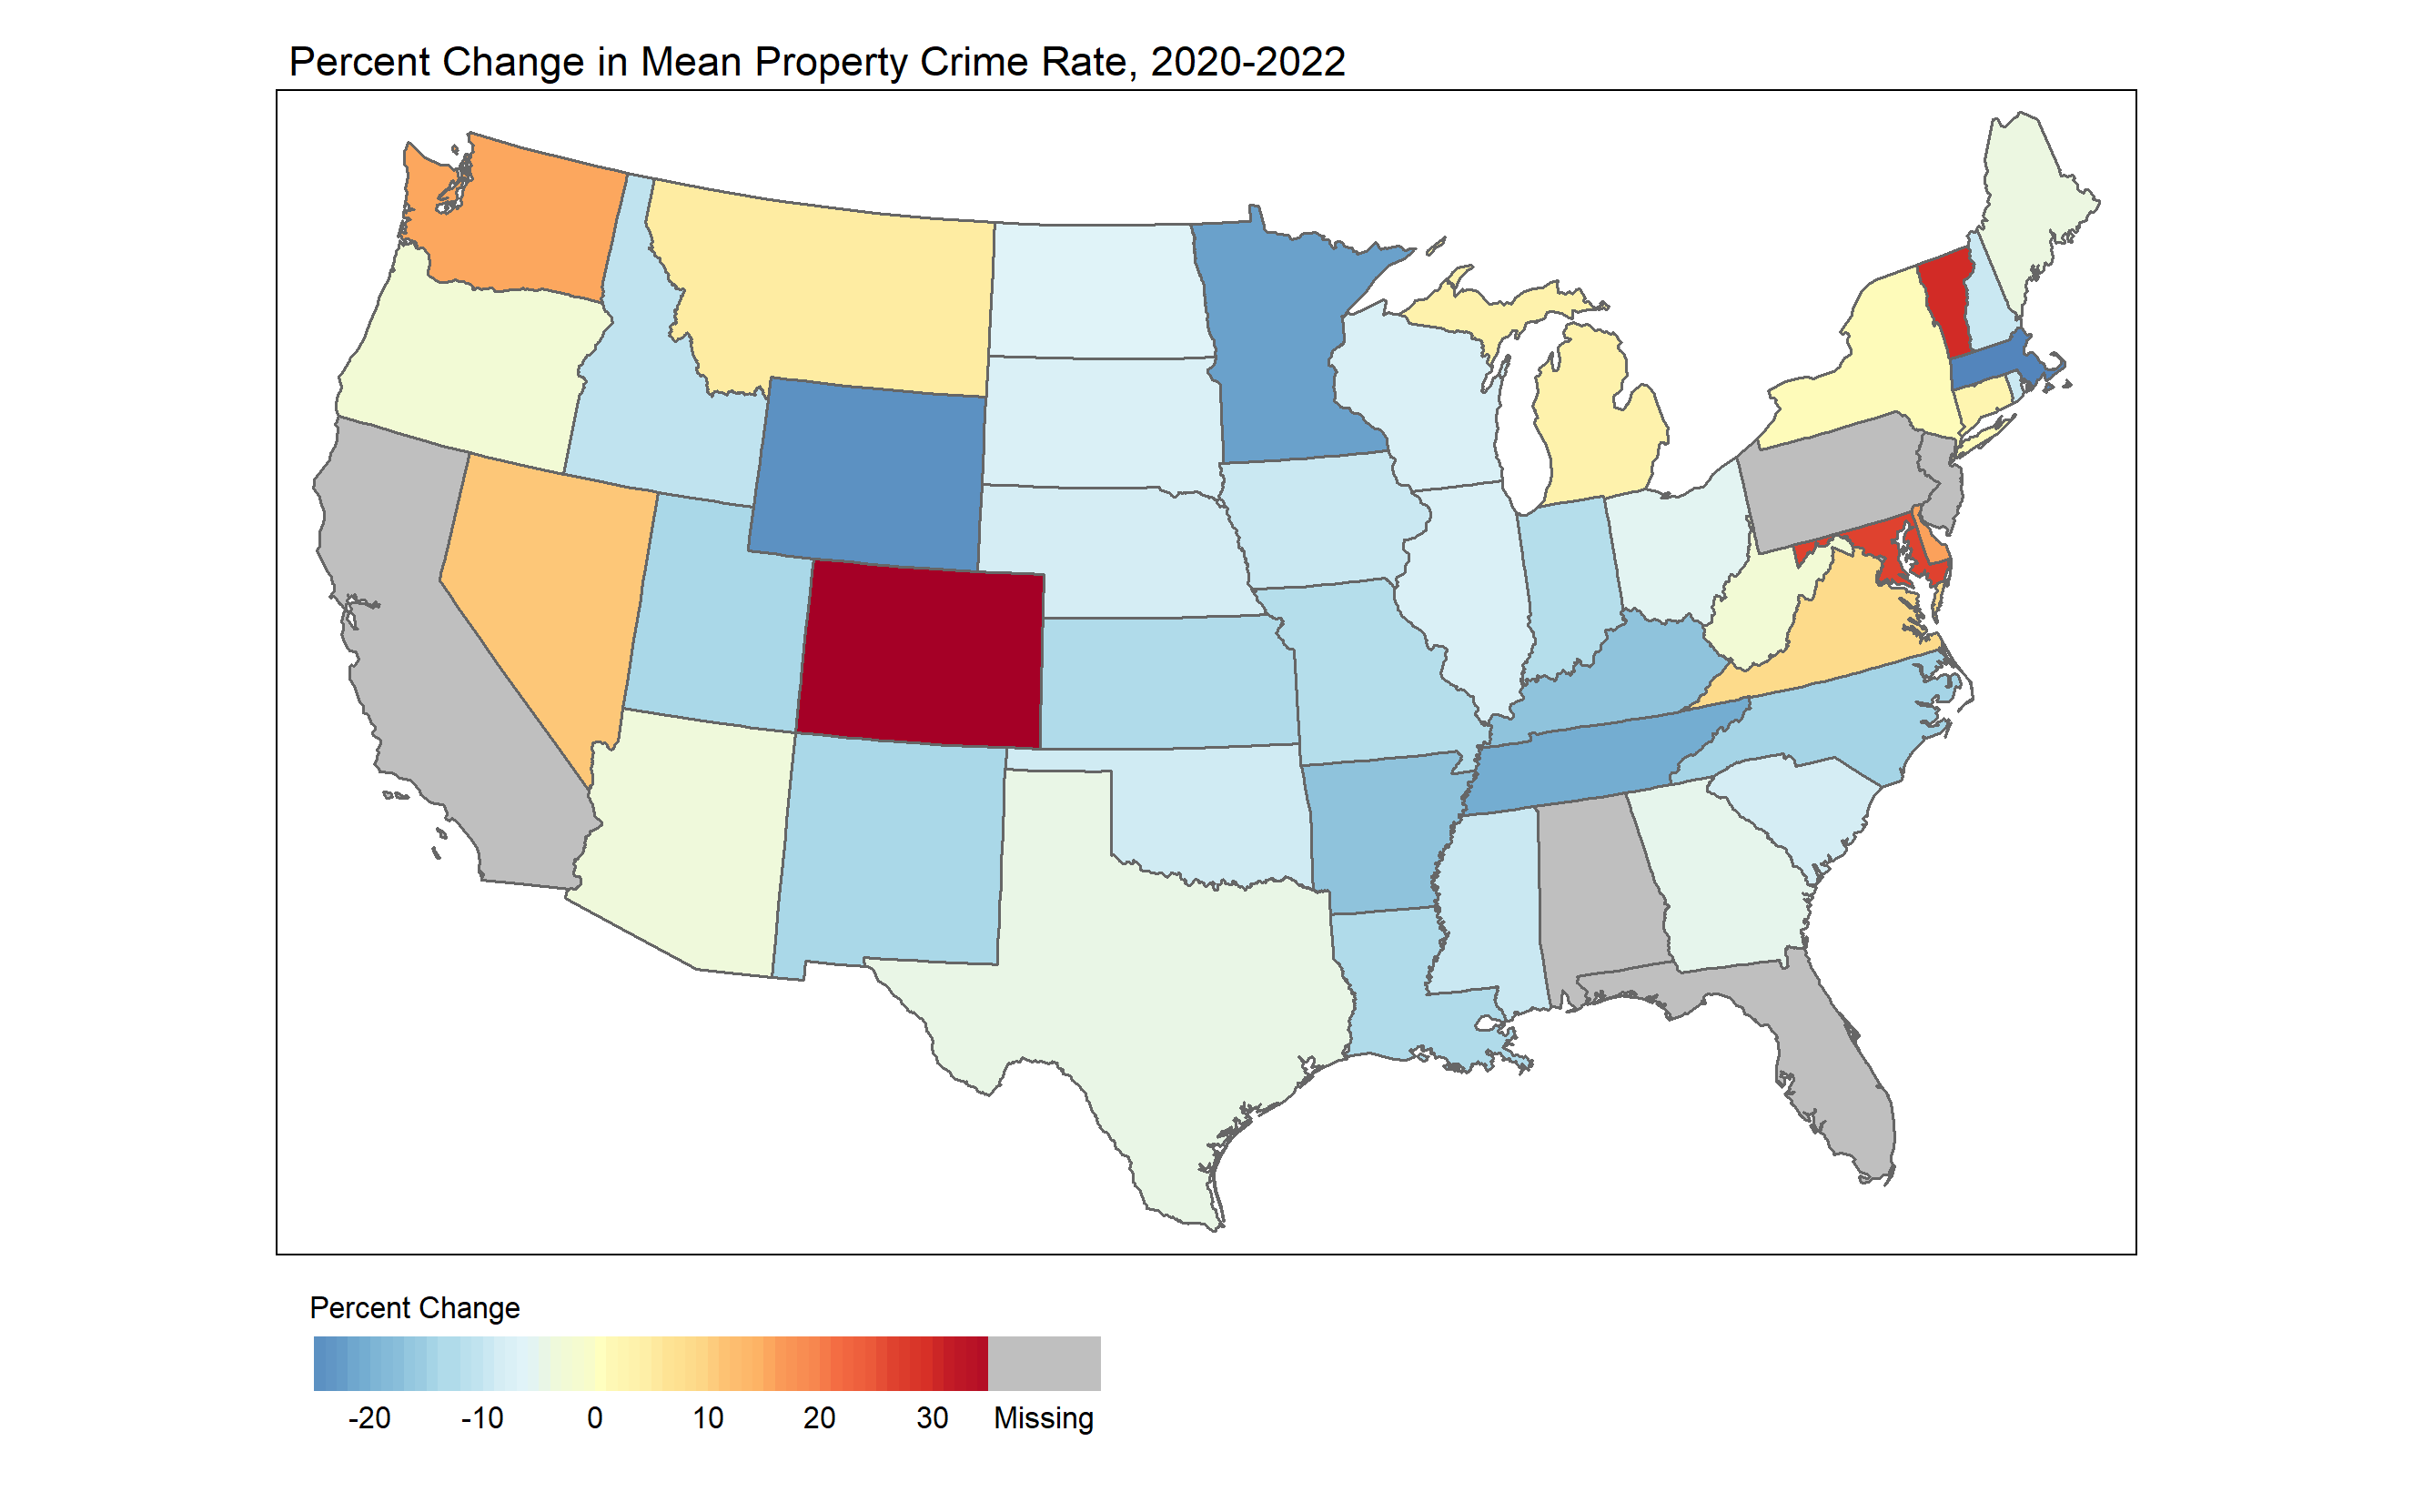
\includegraphics{Plots/States_Property_noPA.png}

The following graphic reports the information shown in the above maps as
a heatmap. Across the board, there was a slight increase in crime rates
from 2020-2023. There are some outliers (most notably Pennsylvania),
which we attribute to either disruptions in data-collection accuracy due
to Covid-19 or the over-representation of low-population cities in
certain states, which could create big swings in crime rates per 1,000
people.

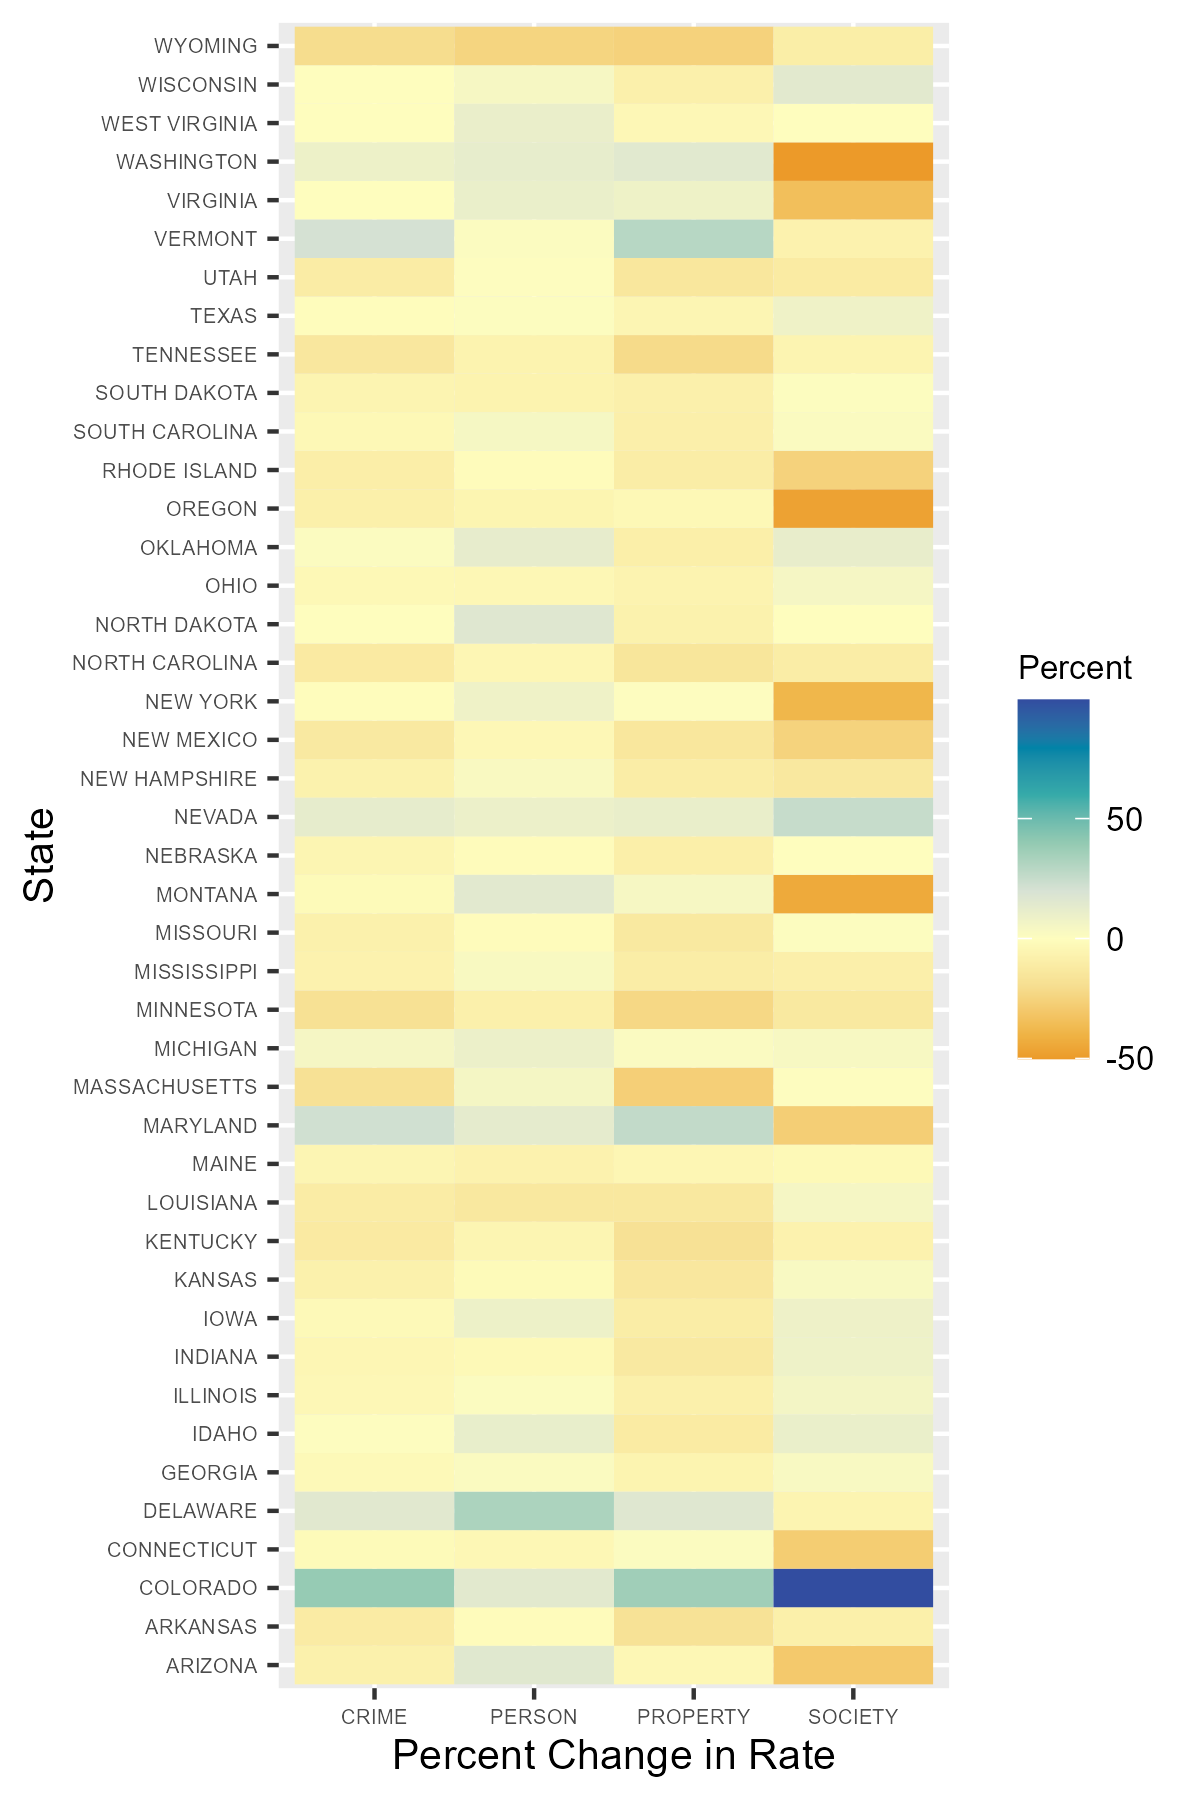
\includegraphics{Plots/States_heat.png}

The cities that enacted zoning reform are concentrated in the Midwest
and Atlantic regions. The map bellow shows these cities and their
populations. The cities that enacted zoning reform tend to skew to
higher populations.

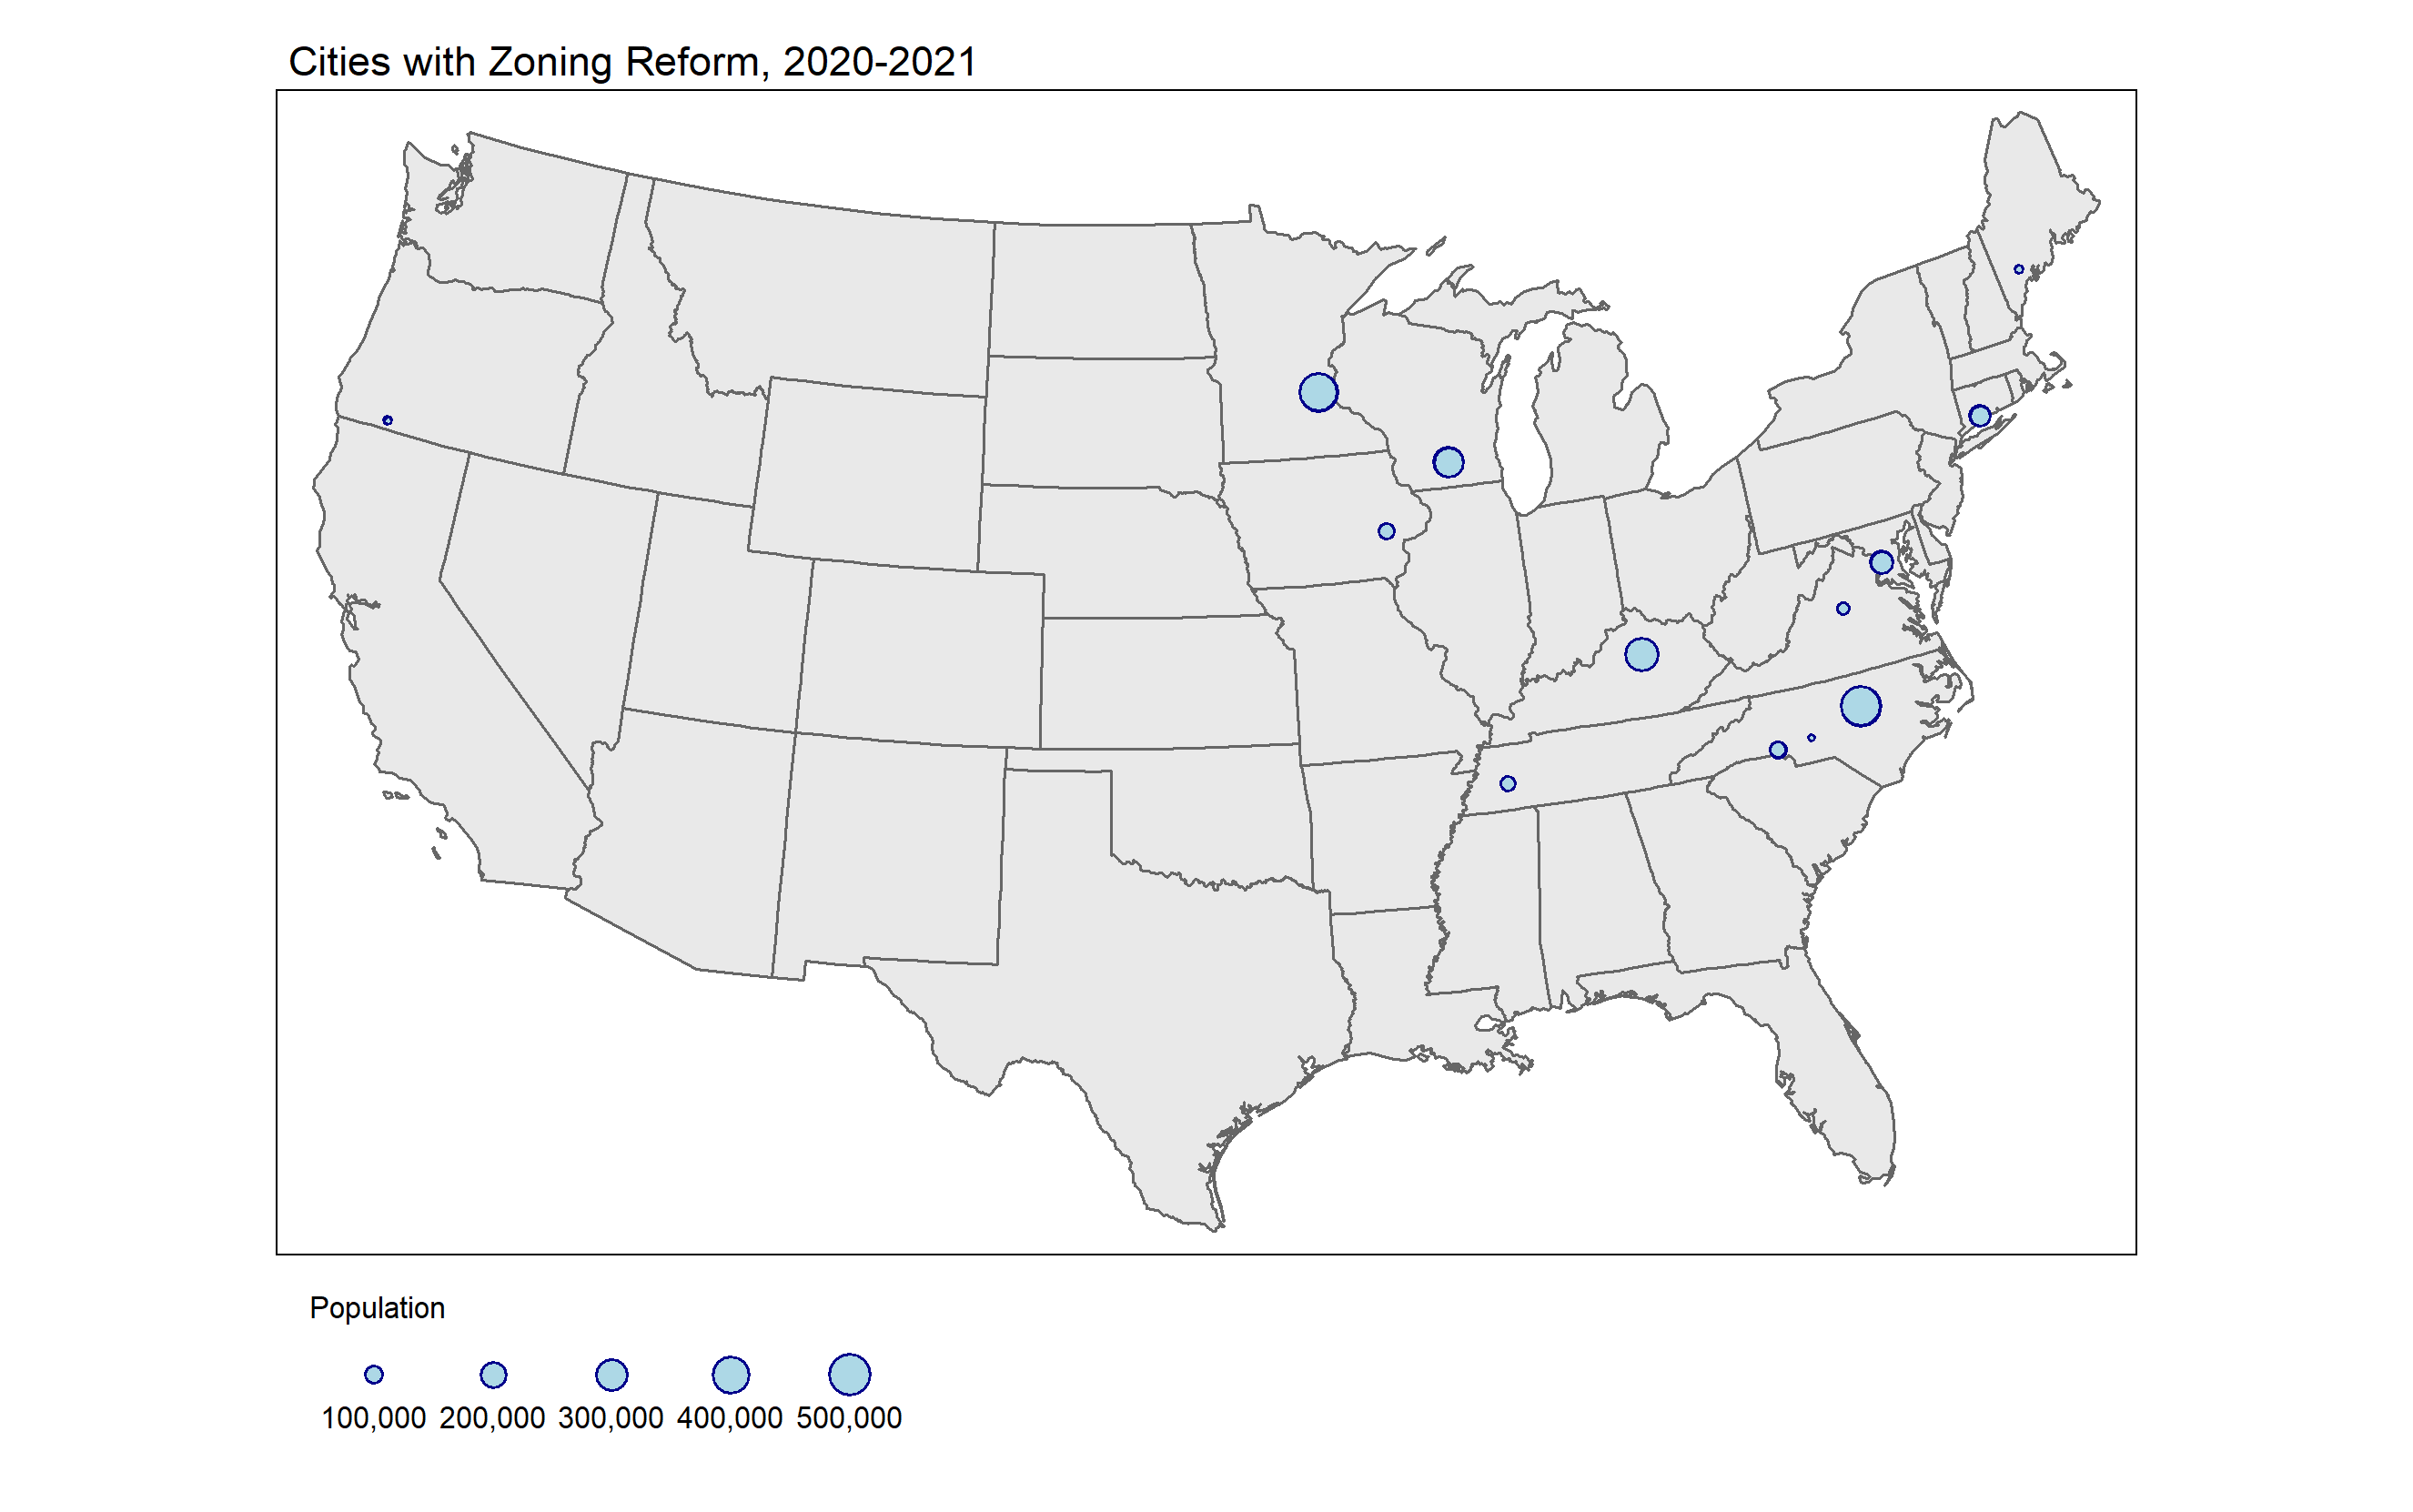
\includegraphics{Plots/Cities_pop.png}

The map below shows the percent change in mean total crime rate for
these cities. We see a fairly even split between cities that saw
increasing total crime rates and cities that saw decreasing total crime
rates.

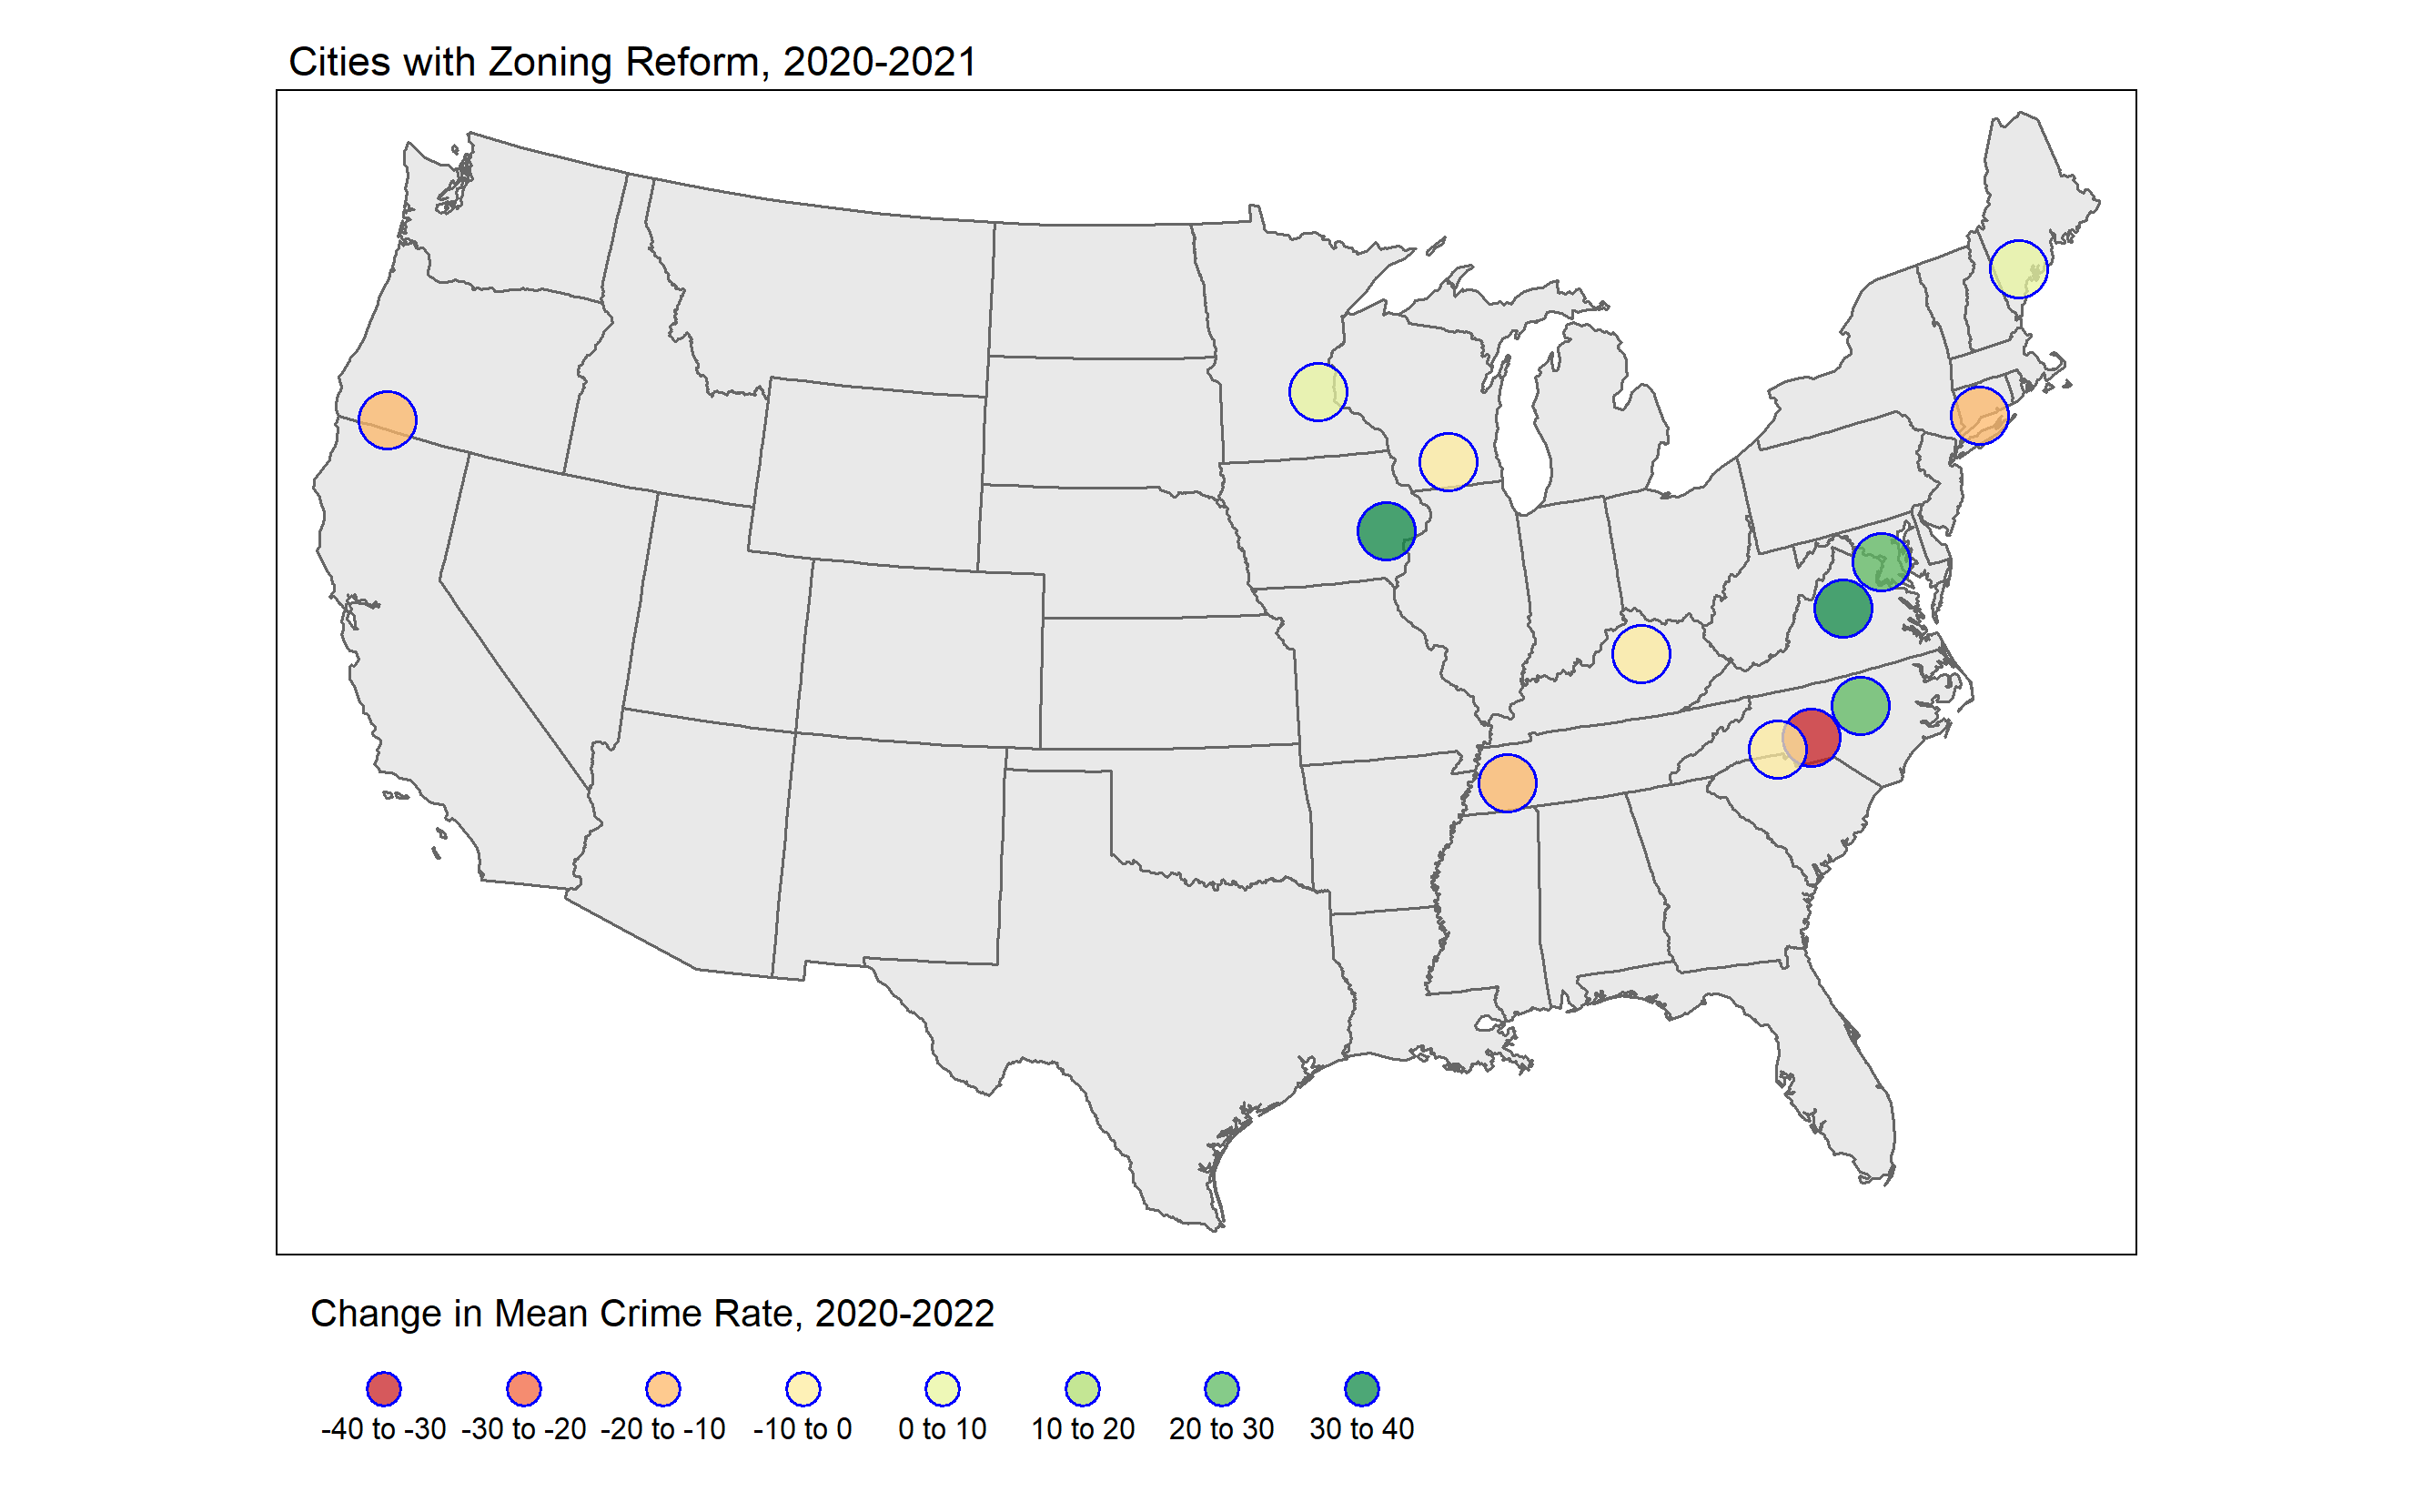
\includegraphics{Plots/Cities_ratechange.png}

The below four scatter-plots in Figure 1 shows the crime rate (total,
society, persons, and property) versus log-transformed population for
all cities in our dataset. Cities with zoning reform are shown in blue.
For visibility purposes, extreme values are excluded from these figures.
As noted prior in this report, cities that enacted zoning reform tend to
skew to higher populations. This is not surprising, as population
growth/high population might create housing demand that is met by a
policy decision such as zoning reform.

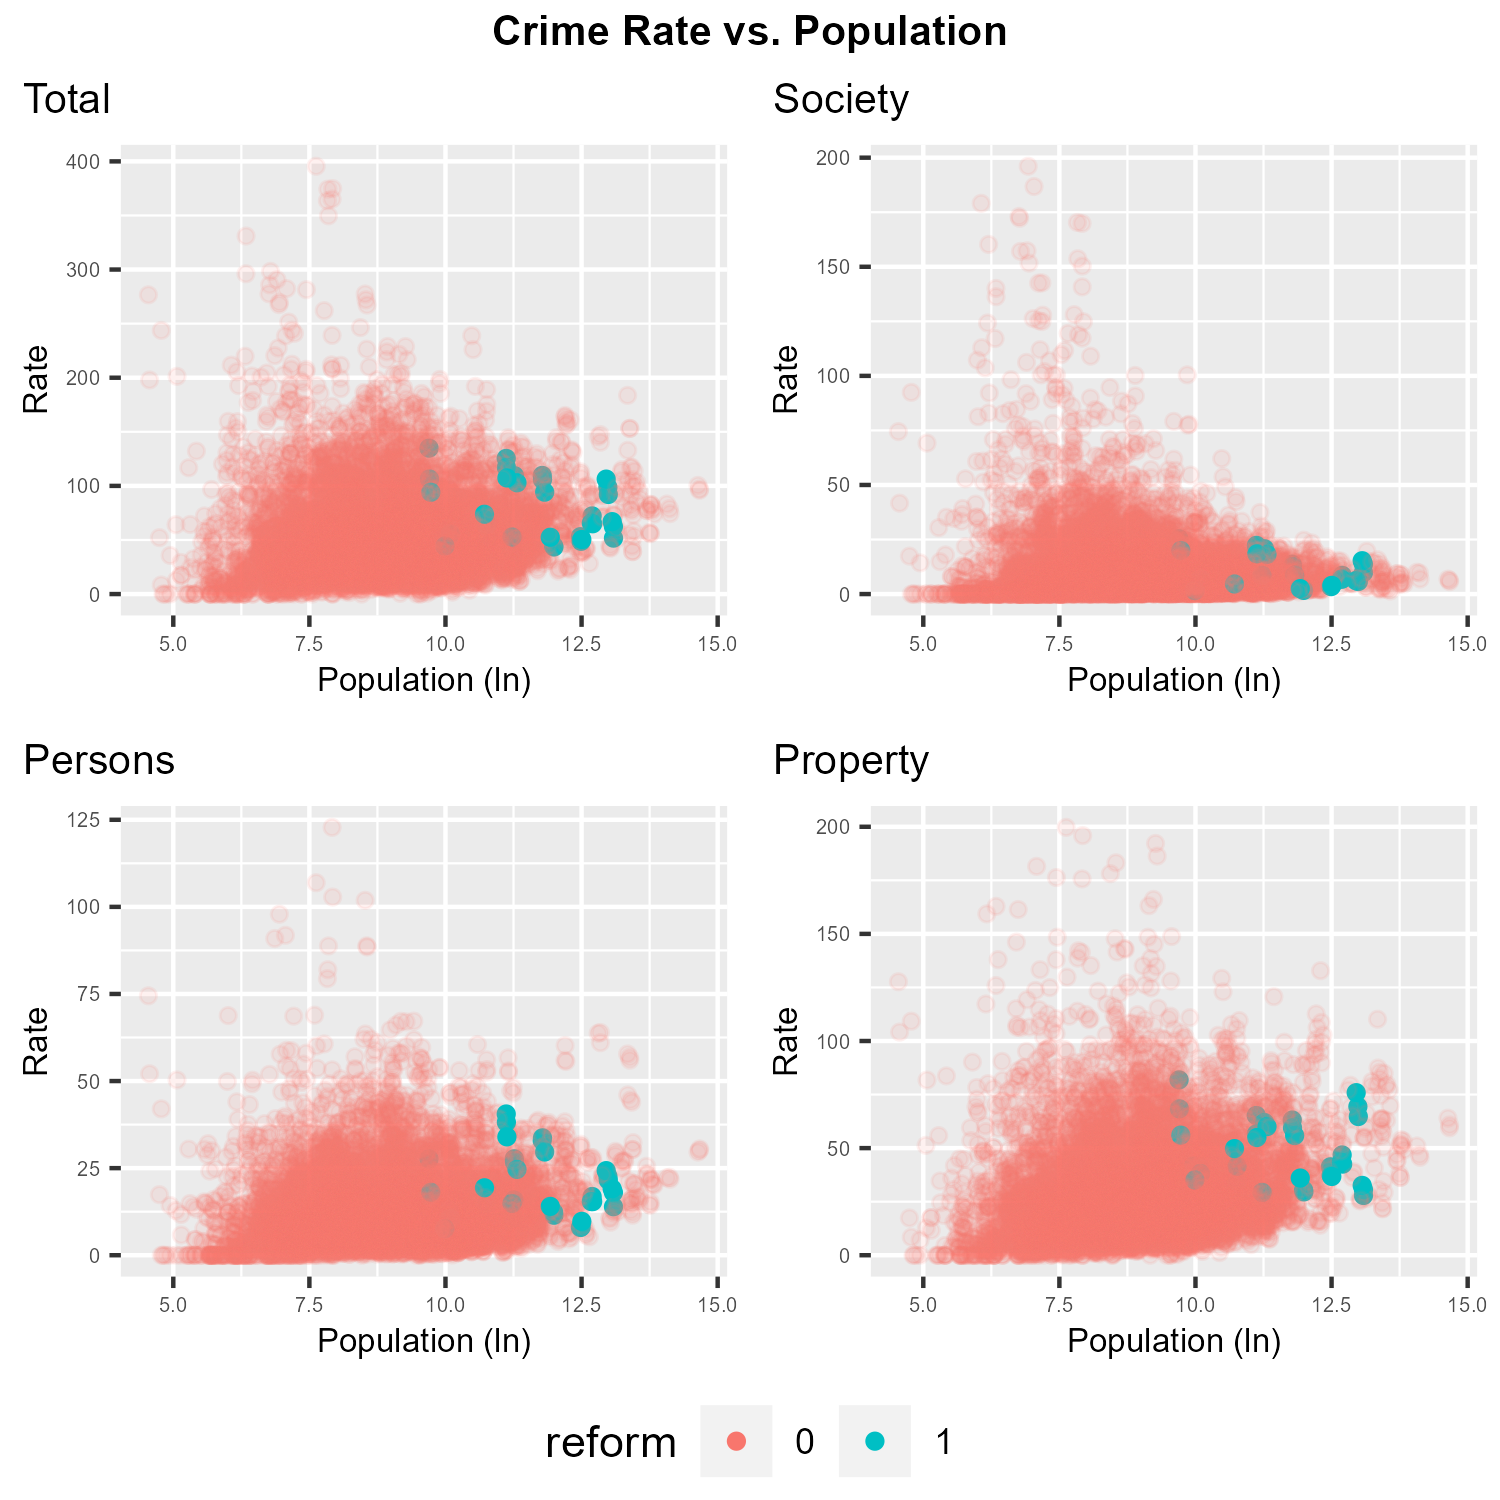
\includegraphics{Plots/Figure1.png}

In Figure 2, the four scatterplots shows the percentage change in crime
rate (total, society, persons, and property) versus log-transformed
population for all cities in our dataset. For visibility purposes,
extreme values are again excluded from these figures.

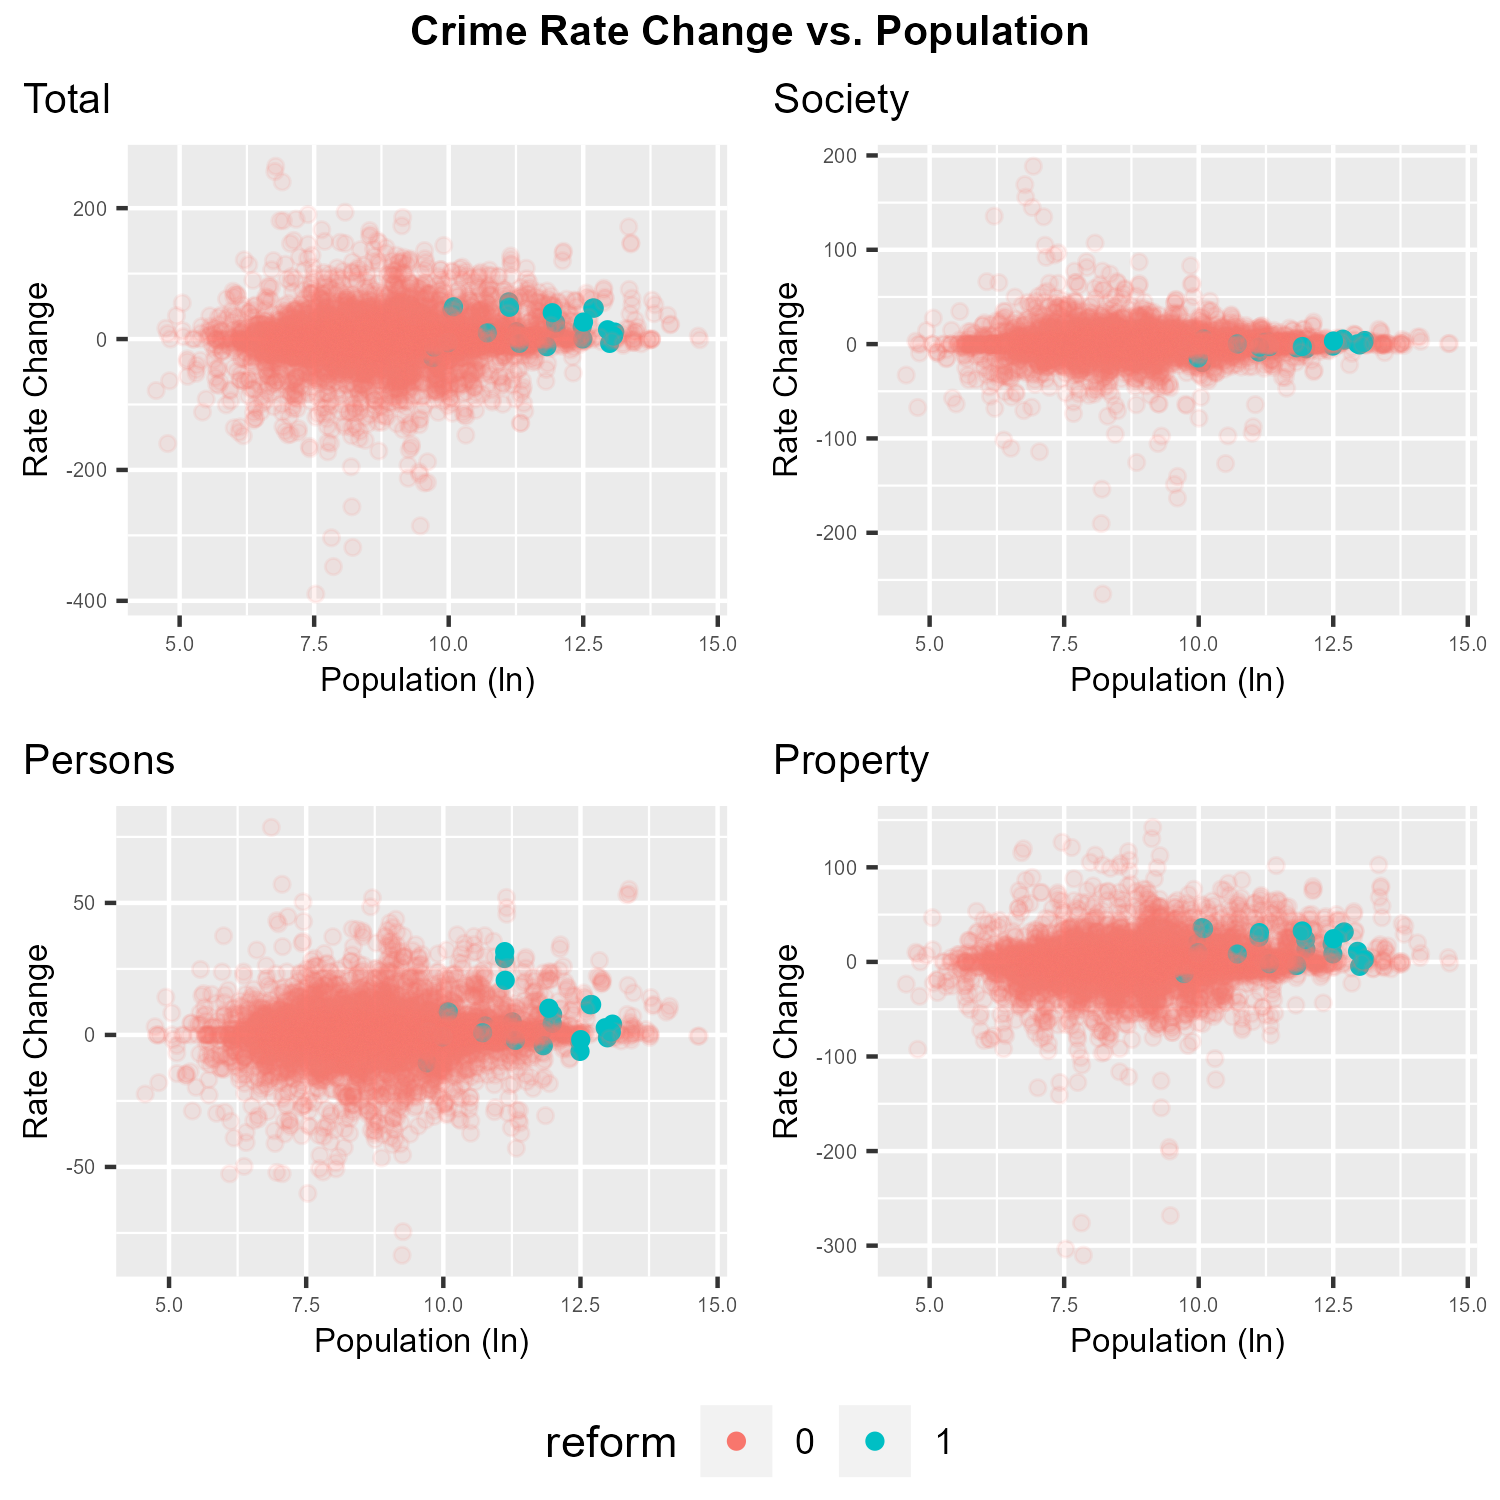
\includegraphics{Plots/Figure2.png}

As is clearly shown in the above graphics, our data is noisy, and there
are also quite a bit of extreme observations. Our data includes cities
with quite low populations, and these cities can have large swings in
crime rate (especially when crime rate is conventionally reported as per
1,000 people). The majority of the data is clustered around 0\%, but the
presence of these extreme observations make visualization tricky. For
the purposes of some of our graphics we have elected to not show these
outliers.

\hypertarget{v.i.-econometric-analysis}{%
\subsubsection{V.I. Econometric
Analysis}\label{v.i.-econometric-analysis}}

\setlength\parindent{24pt}

~~~~~The time frame that zoning reform exists in is far too recent to
make any inferences about the effect of zoning reform on crime. However,
we can describe the cities which have passed zoning reform and determine
if they have a higher crime rate relative to cities which have not
passed zoning reform. This would be important to policy makers, because
if zoning reform is associated with higher crime rates, it would follow
that cities with high crime rates may also have more movements to enact
zoning reform. It would also be useful to future researchers studying
the effects of changes in zoning laws, as findings of significantly
different crime rates and changes in crime rates would impact the
efficiency of their analysis models.

The regression formulas use 4 different dependent variables: total crime
rate, crime rate against property, crime rate against persons and crime
rate against society. These values are reported as the number of crimes
committed per 1,000 people in the agency. The dependent variables are
subdivided in this manner to study the effect of zoning laws on the
kinds of crimes which are committed. The primary independent variable in
question is reform, which is a dummy variable which indicates the
presence of housing reform in that state or city. The control variables
used are the unemployment rate, the mean crime rate for each agency,
which controls for a preexisting level of crime in each city, state
fixed effects, and year fixed effects. An identical set of regression
formulas was run using the change in crime rates as the dependent
variables as well.

Crime Rate = Beta0 + Beta1(Reform) + Beta2(Unemployment Rate) +
Beta3(City Mean Crime Rate) + Alpha(State Fixed Effects) + Gamma(Year
Fixed Effects) + E


\includegraphics{Data/Regression Outputs/pngs/finalchangeregv2.png}

As the regressions show, there is no significant relationship between
crime rates and zoning reform. However, there is a significant
relationship at the 95\% confidence level between zoning reform and
changes in property crime rates and the crimes against persons rate.
What this implies is the impetus for zoning reform may not be an
existing level of crime, but cities where the crime rates for property
crimes and crimes against persons increase sharply. Movements for
housing reform may therefore be associated with shocks in the crime
rate.

A notable issue with the model as shown is that the unemployment rate
for each state decreases the estimated crime rate for each city.
Logically, a higher unemployment rate should be associated with a higher
crime rate, so a negative coefficient for unemployment rate may indicate
issues between it and the mean crime rate. Perhaps the unemployment and
mean crime rate are heavily correlated with each other, which leads to
the confusing value for unemployment rate.

\hypertarget{v.ii.-conclusions}{%
\subsubsection{V.II. Conclusions}\label{v.ii.-conclusions}}

\setlength\parindent{24pt}

~~~~~Although we noted several caveats with our model, our econometric
analysis produced interesting results: the significant relationship
between zoning reform and crime against property and persons. As noted
throught this write-up, there are significant issues with the
simultaneous lack and abundance of data. We have few years of crime
data, and we have magnitudes more data for cities that did not enact
zoning reform. This is also a recent policy change, and the effects of
zoning change are most likely lagged due to the time constraints on
building. While this is an interesting area of analysis, our work here
looks at very preliminary data. Future work will have the luxury of more
extensive data.

We note some final thoughts on limitations for future work. The issue of
the Covid-19 year will still have significant impacts. The lack of
consistently reported crime data during those years do present some
serious difficulties.

Future studies when data of the effects of zoning reform is made
available will be able to note that the environment of the different
cities are defined by a difference in the change of crime rates. This
may make future studies which are relying on a difference in difference
or event time model problematic, since the assumption of parallel
preexisting trends may not hold up in these conditions. Researchers
following up on this subject would do well to account for the different
trends to ensure the accuracy of their findings.

\hypertarget{v.iii.-references}{%
\subsubsection{V.III. References}\label{v.iii.-references}}

Anderson, James M., et al.~``Reducing Crime by Shaping the Built
Environment with Zoning: An Empirical Study of Los Angeles.'' University
of Pennsylvania Law Review, vol.~161, pp.~700-756.

Browning, Christopher R., et al.~``Commercial Density, Residential
Concentration, and Crime: Land Use Patterns and Violence in Neighborhood
Context.'' Journal of Research in Crime and Delinquency, vol.~47, no. 3,
August 2010, pp.~329-357.

Carter, Sherry P., et al.~``Zoning out Crime and Improving Community
Health in Sarasota, Florida: `Crime Prevention Through Environmental
Design'.'' American Journal of Public Health, vol.~93, no. 9, September
2003, pp.~1442-1445.

Crime Data Explorer. ``NIBRS table: State Tables, Offenses by Agency.''
Federal Bureau of Investigations.

Katyal, Neal K. ``Architecture as Crime Control.'' The Yale Law Journal,
vol.~111, pp.~1039 -1139.

Meyersohn, Nathaniel. ``The Invisible Laws that Lead to America's
Housing Crisis.'' CNN Business. August 5, 2023. Available from:
\url{https://www.cnn.com/2023/08/05/business/single-family-zoning-laws/index.html}.

Othering \& Belonging Institute. ``Zoning Reform Tracker.'' University
of California, Berkely. Available from:
\url{https://belonging.berkeley.edu/zoning-reform-tracker}.

Hlavac, Marek (2022). stargazer: Well-Formatted Regression and Summary
Statistics Tables. R package version 5.2.3.
\url{https://CRAN.R-project.org/package=stargazer}

United States Department of Agriculture. (n.d.). County-level data sets.
USDA ERS - County-level Data Sets.
\url{https://www.ers.usda.gov/data-products/county-level-data-sets/}

\end{document}
